\section{Earlier 1K adaptation and its 16K extrapolation failure}
\label{app:context-study}
This completed experiment precedes the matched 16K distance intervention in
Section~\ref{sec:distance-design}. Its evaluation seed, prompts, adaptation
budget, and timing panel differ. Its numerical results are retained separately
and are not substituted into the later matched quality--cost comparison.

\subsection{Earlier selection and frozen evaluation}
The earlier three-seed campaign learns the paired posterior only for seed 71;
seeds 53 and 89 remain near chance. We therefore explicitly select the fixed
seed-71 independent terminal checkpoint for a conditional mechanism study,
while retaining all six outcomes. A fresh eight-condition development probe
first checks short competence, then measures every long-context cell.
The one bounded follow-up preserves the task and labelled output format:
200 fixed updates at global batch 32, learning rate $10^{-5}$ with 20-update
warmup, using 25\% short and 75\% 1K inputs and the original independent paired
information-set objective. Its discarded 20-update GPU qualification passes
on all eight ranks. All 2,500 auxiliary training updates remain part of the
model's history; adaptation starts with a fresh optimizer.

Before evaluating these two fixed checkpoints, we freeze 16 base problems
per family, test seed 20271001, all ten length/position cells, and both fixed
checkpoint selectors: the original model and its terminal 200-update
adaptation. Every cell is retained regardless of short-task performance.
The test structure catalog was used in the earlier campaign, so this is a
fresh-condition assessment within a previously observed held-out catalog,
conditional on a selected training lineage. It is not an untouched-structure
test or evidence about reliability across training seeds.

The earlier study's primary estimand is information-set improvement over one call in paired
parity at 16K, averaging the three evidence positions within each base problem.
We also report the equal-call contrast, valid mass, all cells, and each gain's
interaction with short context. Pointwise 95\% percentile intervals use
10,000 bootstrap draws over base problems, retaining all policies, lengths,
positions, and both checkpoints together. No endpoints are discarded and no
sample extension depends on significance. All 640 conditions across the two checkpoints are complete and validated.
Exact public prompts have no overlap with the earlier confirmation panel
or the eight-condition development probe.

\subsection{Results of the earlier adaptation}
\paragraph{Learning at the trained length does not ensure extrapolation.}
Before context adaptation, paired-parity information-set KL is 0.0407 nats
on the fresh short-input panel. At 1K, it rises to 28.53 and 29.66 for far and
middle public blocks, while remaining 0.383 for nearby blocks. The fixed
200-update adaptation reduces these 1K errors to 0.0127, 0.0185, and 0.0121,
with valid mass 0.9922, 0.9897, and 0.9928. Thus the model can learn useful
conditional predictions at the trained length.

At 4K, adapted information-set KL is 1.842, 0.992, and 0.148 for far, middle,
and near placements. The mean gains over one call are positive, but the
far-position gain interval includes zero: 0.931 nats with interval
$[-0.587,2.046]$. At 16K, information-set KL rises to 21.83, 21.41, and 3.245.
Figure~\ref{fig:final} retains every length and position. Improving in-distribution
conditional predictions does not imply that the same error budget holds at
a longer, untrained context length.

\begin{figure}[t]
\centering
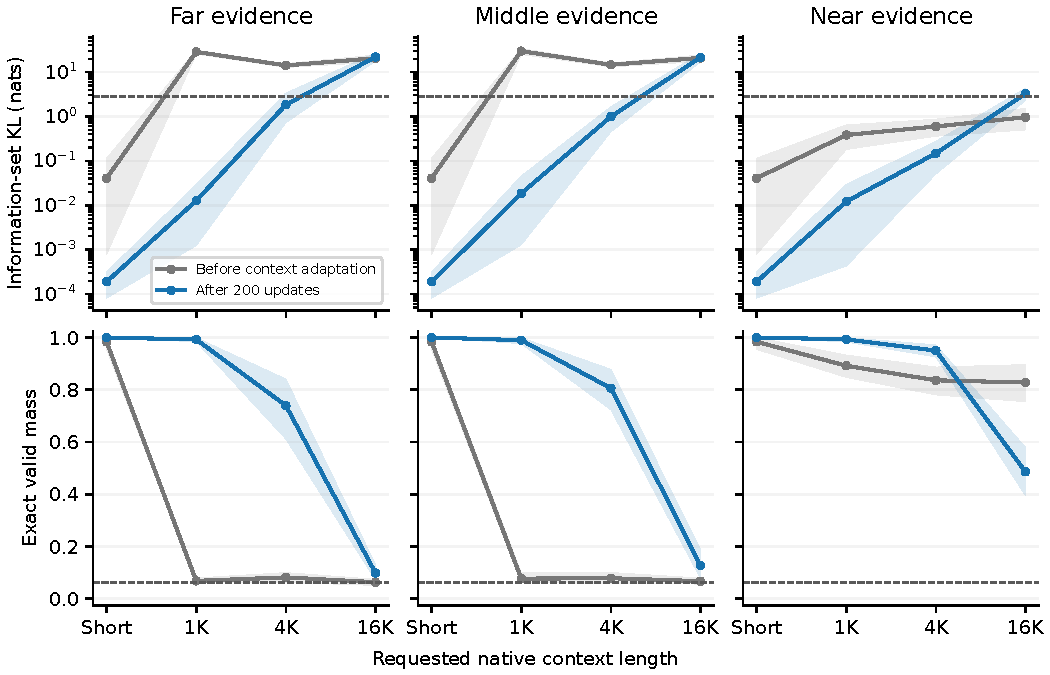
\includegraphics[width=\linewidth]{results/posterior_context_final/mechanism_final.pdf}
\caption{Frozen fresh-condition results for the information-set policy.
Each cell averages 16 paired-parity problems; bands are pointwise 95\%
problem-bootstrap intervals. The dashed KL line is the one-call product
lower bound $4\log2$, and the dashed validity line is $1/16$.
Both checkpoints share the selected seed-71 training lineage.}
\label{fig:final}
\end{figure}

\paragraph{The primary 16K criterion fails.}
Averaging evidence positions within each problem, two calls worsen KL relative
to one call by 11.309 nats before adaptation and 12.723 afterward
(Table~\ref{tab:primary}). Both paired intervals exclude zero in the unfavorable
direction. The adaptation's change in two-call KL itself is inconclusive at
this aggregate: KL reduction $-1.390$, interval $[-5.448,2.678]$.
We do not interpret a larger point estimate as a reliable overall degradation.

\begin{table}[t]
\centering\small
\caption{Predeclared 16K paired-parity aggregate, equally weighting positions
within each of 16 problems. KL gain is one-call minus two-call KL;
positive is favorable. Intervals concern problems, not training seeds.}
\resizebox{\linewidth}{!}{\begin{tabular}{@{}lrrrrl@{}}
\toprule
Checkpoint & One-call KL & Two-call KL & Two-call validity & KL gain & 95\% interval\\
\midrule
Before adaptation & 2.797 & 14.106 & 0.319 & -11.309 & $[-13.620,-8.873]$\\
After adaptation & 2.773 & 15.496 & 0.237 & -12.723 & $[-15.808,-9.968]$\\
\bottomrule
\end{tabular}
}
\label{tab:primary}
\end{table}

Validity alone gives a different impression. Two calls increase average valid
mass over one call by 0.257 before adaptation and 0.175 afterward, despite the
worse forward KL. A model can put appreciable mass on valid answers while
strongly distorting their uniform target distribution. Reporting within-valid
KL and full endpoint KL prevents this from being mistaken for a better
posterior sampler.

The equal-call intact-pair control also illustrates the role of estimation.
After adaptation, the information-set policy improves mean 16K KL over that
control by 18.685 nats, interval $[16.326,21.392]$. Only $4\log2=2.773$ nats
of this contrast is the prescribed dependence reduction; the remaining
15.912 nats is the difference in learned estimation errors. Thus the
same-call intervention does not isolate dependence error alone.
The successful information-set histories and poorly learned alternative
histories are consistent with the coverage analysis, without proving a
particular internal cause.

\paragraph{Matched-task cost conditions hold; the quality certificate does not.}
Before collecting these timings or observing the adapted final outcomes, we
fix a 1.5-second mean-request budget. The cost check uses the same 16
paired-parity problems and three 16K placements, with one separate warmup and
ten complete timed requests per condition and policy. The recurrent checkpoint
is the fixed 200-update adaptation; the Pythia adapter is its previously
qualified 20-update checkpoint. Attention accuracy is not measured: the
comparison uses the analytic lower bound for any one-call product sampler.

Mean recurrent latencies are 0.650 seconds for one call and 1.300 seconds for
the information-set two-call policy. Attention takes 1.000 and 1.998 seconds,
respectively; its intact-pair two-call policy takes 1.999 seconds. The
pointwise problem-bootstrap intervals for the information-set costs are
$[1.298,1.302]$ and $[1.993,2.004]$ seconds. Hence the predeclared budget permits
recurrent two-call and attention one-call execution while excluding both
other declared attention policies. Nevertheless recurrent mean KL is 15.496,
well above the $4\log2=2.773$ sufficient threshold. The empirical-panel
certificate fails its quality condition. This failure does not determine the
unmeasured attention model's actual KL.

These are mean-cost measurements, not per-request deadline or broad population
guarantees. Peak allocated memory is 4.125 GiB for recurrent two-call execution
and 2.234 GiB for attention; this implementation establishes no memory advantage.
The earlier auxiliary screen finds attention faster at 1K and 4K and cached
causal RWKV cheaper at 16K (Appendix~\ref{app:lookup}); a linear arithmetic
count alone does not imply universal speed superiority.

